\begin{frame}{Signal VS WhatsApp VS Telegram}
    \framesubtitle{WhatsApp}

    \textbf{Pro}
    \begin{itemize}
        \item Crittografia end-to-end per chat, video, gruppi, chiamate, fotografie
        \item Implementa il protocollo Signal (l'implementazione in sé è closed-source)
        \item Interfaccia parzialmente personalizzabile
        \item 2 miliardi di utenti attivi
        \item Supporta autenticazione a due fattori
    \end{itemize}\pause

    \textbf{Contro}
    \begin{itemize}
        \item Poche impostazioni sulla privacy
        \item Raccolta dati utente per fini di marketing
        \item Backup basati su cloud non crittografati, metadati non crittografati
    \end{itemize}

    \note{
        Informazioni raccolte: numero di telefono, posizione, contatti, abitudini, cronologia di navigazione, cronologia acquisti, dati pubblicitari, ID utente e dispositivo, indirizzo e-mail, informazioni di pagamento, dati sulle prestazioni e altri contenuti utente\newline
        Recente (2019) problema di WhatsApp ha coinvolto numerose chat di gruppo i cui link erano disponibili tramite ricerca Google [bug eliminato a febbraio 2020]
    }
\end{frame}

\begin{frame}{Signal VS WhatsApp VS Telegram}
    \framesubtitle{WhatsApp}
    WhatsApp implementa il protocollo Signal basandosi sulle librerie open-source:
    \href{http://github.com/whispersystems/libsignal-protocol-java/}{GitHub - WhatsApp}\newline\pause

    \begin{figure}
        \centering
        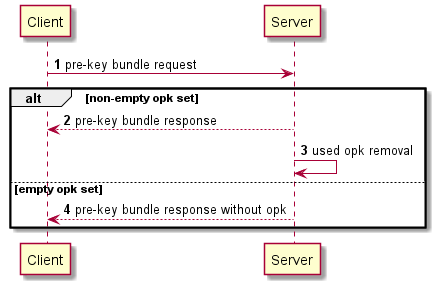
\includegraphics[width=.5\textwidth]{whatsapp session initiation.png}
        \caption{WhatsApp inizializzazione sessione (singolo dispositivo)}
        \label{tag: wa session initiation}
    \end{figure}
    
\end{frame}